%!TEX root = kotov.tex
\section{Task 4}
\begin{task}
    Даны два массива из положительных чисел $a$ и $b$, размер обоих равен $n$. Выбрать массив $p$ из $k$ различных чисел от $1$ до $n$ так, чтобы $\frac{\sum_{i=1}^ka_i}{\sum_{i=1}^kb_i}\to\text{max}$. Время $\O(n\log M)$, где $M =\max\limits_i(a_i/b_i)$.
\end{task}

\begin{solution}
    Ряд информации, взятой из общего чата: $M=\max\limits_i(a_i,b_i,n)$, числа помимо того, что положительные еще и целые.
    Рассмотрим $\sum_{i\in I} a_{i} / \sum_{i\in I} b_i \geq t$, где $I$ некое $k$-элементное подмножество из $[1,\ldots,n]$. Это отношение можно переписать в виде: $S = \sum_{i\in I} a_{i} - t\sum_{i\in I} b_i \geq 0$. То есть зададимся вопросом, есть ли такое $I$, что эта разность верна для какого-то заданного $t$?
    
    Рассмотрим множество $\{a_i - tb_i\}_{i=1}^n$. Найдем $n-k$-ую порядковую статистику в этом множестве (то есть хотим найти элемент, который бы стоял на $k$-ом месте в отсортированном по убыванию массиве). Возьмем все элементы, начиная с этого и до конца массива вправо в качестве искомых. Если для таких элементов $S<0$, то для такого $t$ не существует никакого $I$, чтобы $S\geq 0$, так как все оставшиеся элементы заведомо меньше уже взятых, значит, если бы мы взяли кого-то из них, то результирующая $S$ была бы еще меньше. С другой стороны, если для данного $t$ $S\geq0$, то мы получили какой-то набор элементов.
    
    Что мы в действительности хотим, так это как можно больше увеличить $t$. Было бы неплохо понять, какие границы может принимать $t$: из очевидного, можно за левую границу взять $t=0$, а за правую $t=\max(a_i/b_i)$.
    \begin{remark}
        Рассмотрим, почему такая правая граница подойдет. Рассмотрим индивидуальные дроби $\frac{a_i}{b_i}$. Обозначим наибольшую из них как $\frac{a}{b}$. Посмотрим, как относятся друг с другом $\frac{a}{b}\lessgtr\frac{a+x}{b+y}$, где $x/y$ какая-то другая дробь из оставшихся.
        \begin{gather}
            \frac{a}{b} - \frac{a+x}{b+y} = \frac{ay-bx}{b(b+y)}
        \end{gather}
        Нас интересует знак этого выражения. Так как знаменатель строго положителен, то остается рассмотреть $ay-bx \lessgtr 0$.
        Для этого вспомним, что $a/b$ --- наибольшая дробь, то есть, в частности, $\frac{a}{b} > \frac{x}{y}$, следовательно, $ay > bx$. Таким образом, ``прибавление'' какой угодно дроби к наибольшей уменьшает отношение.
    \end{remark}
    \begin{remark}
        Если рассмотреть $S$ как функцию от $t$ при фиксированном $I$, то это будет монотонная убывающая функция, что полезно для бинпоиска.
    \end{remark}
    То есть на данный момент, мы умеем выбирать потенциальный набор $I$ за $\O(n)$ для всякого $t$. А вот с бинпоиском теперь наступают проблемсы, если для старого $M$ это было бы ответом, так как мы бы за $\O(\log \max(a_i/b_i))$ находили бы нужный $t$ и в результате получили бы сложность $\O(n\log M)$, то с новой $M$ не совсем понятно, откуда здесь взять эти штуки. Казалось бы, $t$ у нас реально может принимать только рациональные значения, а их на конечном промежутке конечно, можно замапить, видимо, это отношения на числитель/знаменатель/количество элементов. С другой стороны, я понимаю, почему концептуально может не работать старое $M$ (хотя бы потому, что $\log M\Big|_{M=1} =0 $)
    \begin{upd}
        Вспомним, что рациональные числа на конечном промежутке конечны. Тогда рассмотрим, какие возможные дроби мы можем получать для исходных $a$ и $b$. Рассмотрим грубую оценку, когда мы не ограничены только лишь суммами соответствующих пар, то есть всевозможные отношения сумм. Наименьший возможный числитель для таких дробей --- это $1$, а наибольший $\sum\limits_{i=1}^na_i$, аналогично и для $b_i$. В случае, когда у нас нет ни одного элемента, превышающего $n$, то это значит, все $a$ либо принимают значения $[1,\ldots,n]$ либо некоторые (возможно все) из них совпадают, это же верно и для $b$.

        Если же $a$ содержит элемент(ы), превосходящие $n$, то ничего особо полезного сказать нельзя, разве что числитель индивидуальных дробей ограничен $\max\limits_i(a_i)$.
        
        Теперь составим змейку, пересчитывающую рациональные числа
        \begin{figure}[H]
            \centering
            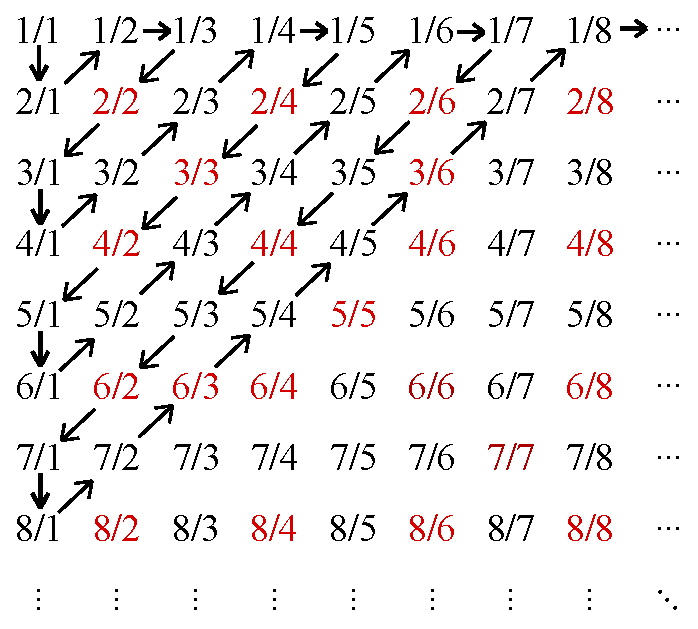
\includegraphics[scale=0.7]{pics/Diagonal_argument.eps}
            \caption{Пересчет рациональных чисел}
        \end{figure}

        Пусть мы отсортировали пары $(a_i, b_i)$ по первому ключу. Тогда, мы можем начинать отсчитывать вертикаль от $a_1$, а заканчивать вертикаль $a_n$, горизонталь из $b_i$ сформируем в том порядке, в котором выставлены соответствующие $a_i$.
        \begin{enumerate}[1)]
            \item 
            Тогда, если никакие $a_i$ и $b_i$ не превосходят $n$, то наибольшее достижимое значение числителя и знаменателя мы можем ограничить как $Cn$, где $C$ константа. Бинпоиск же интересующего нас $t$ можно организовать среди диагональных элементов такой увеличенной матрицы $Cn \times Cn$, то есть среди $Cn$ штук элементов.
            \item
            Теперь случай когда, у нас могут быть элементы б\'ольшие $n$. В этом случае, мы уже говорил, что $t$ реально ограничено $\max(a_i/b_i)$. То есть если мы составим расширенную матрицу размера $max(a_i, b_i) \times \max(a_i, b_i)$ (содержащую ту структуру с отсортированными элементами $a_i$), то среди диагональных элементов этой матрицы будет где-то находится искомое $t$.
        \end{enumerate}
        Таким образом, реально ведется поиск среди элементов таких диагоналей, а их количество ограничивается (без учета съедаемой слабой асимптотики для случая, когда $n > \max(a_i, b_i)$) $\max(a_i, b_i, n)$.
        Таким образом, окончательно приходим к ответы для исправленной $M$.
    \end{upd}
    \begin{upd}
        В целом, судя по этой процедуре, мы можем один раз предрасчитать массив рациональных числе за $\O(n\log M)$, а затем уже обращаться к этому массиву (предварительно отсортированном), то есть результирующая сложность хуже, в смысле О-большого, не стала.
        Так же можно посмотреть на то, что предлагают авторы этой статьи \cite{KWEK200323}.
    \end{upd}
\end{solution}